\pdfoutput=1
\documentclass[11pt]{article}
\usepackage[margin=1in]{geometry}
\usepackage[T1]{fontenc}
\usepackage{lmodern}
\usepackage{amsmath}
\usepackage{booktabs}
\usepackage{graphicx}
\usepackage{float}
\usepackage{caption}
\captionsetup[table]{position=top,skip=6pt}
\usepackage{tabularx}
\usepackage{xcolor}
\usepackage[numbers,sort&compress]{natbib}
\usepackage[hidelinks]{hyperref}

\newcommand{\sig}{\ensuremath{^{*}}}
\newcommand{\todo}[1]{\textcolor{red}{[TODO: #1]}}

\title{Can the Other Side Steer Your AI Lawyer?\\
\large Prompt Injection, Framing and Record Manipulation in AI Legal Review}
\author{Jay Cho\thanks{The author is a practising solicitor admitted in New South Wales, Australia.
This is independent research, done on the author's own time with the author's own resources and
not reviewed by any employer. The views expressed are the author's alone and should not be
attributed to any entity with which the author is associated. Nothing in this paper is legal
advice.}\\
\small Independent researcher\\
\small\texttt{jae.cho.890@gmail.com}}
\date{November 2026}

\begin{document}
\maketitle

\begin{abstract}
Lawyers increasingly run AI reviewers over documents that the opposing party wrote. That party can
place text in those documents meant for the machine rather than for the human reader. We test
whether such text shifts the conclusions of the reviewing party's AI, across four studies, 17
models and about 12,000 assessments, on fictional fixtures drafted by an AI assistant to a lawyer's specification.
(1)~In contract review, explicit and hidden injected instructions (including invisible text in a
real PDF) and authority and sycophancy framing moved frontier CLI-accessed models by at most
2.2 points on a 32-point skew scale, and most models named the injected instruction in most
reviews. One open-weight API model followed the injected instruction by $+20.8$ points.
(2)~In an assessment that unfolds item by item, the order of the evidence dominated: putting one
side's items last moved the final answer toward that side in 22 of 23 model-case cells, and
putting them first moved it away. Slanted per-item glosses moved some models and pushed others in
the opposite direction. (3)~In an IP-assignment assessment, a party's assertions alone almost never
moved the final answer toward that party, but an adversarial bundle that curated, misstated and directed the record
moved every model, in both a negative and a positive-control case. (4)~In a two-stage due-diligence
pipeline, injected claims never survived, but terse summarisation removed the hedges from
uncertain claims, and some deciding models hardened them into firm statements. The threat to AI
legal review is less ``ignore your instructions'' than control of what the record shows and in what
order. All fixtures, prompts, raw records and analysis code are released at
\url{https://github.com/jaecho890-svg/legal-injection-paper}.
\end{abstract}

\section{Introduction}

A buyer's lawyer who asks an AI system to review the seller's draft share sale agreement is
asking a model to read text written by an adversary. The same is true of a litigator reviewing a
document production, an in-house team assessing a counterparty's correspondence, or a deal team
whose AI pipeline summarises a data room before a stronger model decides. In each case the
opposing party controls some of the input, and may write it for the machine.

Indirect prompt injection, in which instructions hidden in retrieved content hijack a model, is
well documented in general settings \citep{greshake2023,perez2022ignore,liu2023injection}. Legal
work adds two features. First, the adversary's text is not incidental content but the very
material under review, so the reviewer cannot simply ignore it. Second, legal conclusions depend on
characterisation, emphasis and the completeness of the record, so an adversary need not issue an
instruction at all: framing, ordering and selective presentation may be enough.

We ask whether text placed by one party shifts the conclusions of the other party's AI reviewer,
and through which mechanism. We separate three families of manipulation:
\emph{injection} (instructions addressed to the AI, visible or hidden), \emph{framing} (authority
claims, anchoring, sycophancy scaffolds, slanted glosses and ordering, with the evidence unchanged)
and \emph{record manipulation} (omitting, misstating or curating the evidence itself). We measure
each against the same model's clean control, with replicates, blinded automated coding validated
against a lawyer's blind coding, and multiple-comparison correction.

Our main findings:
\begin{itemize}
  \item Frontier models accessed through their vendors' CLIs were robust to injection and framing
        in contract review (largest shift 2.2 of 32 points) and usually said what they had seen.
        One open-weight model was not ($+20.8$).
  \item In sequential assessment, evidence order acted through recency, consistently across 13
        models and three cases, and some models reacted against slanted glosses rather than with them.
  \item Assertion alone almost never moved IP conclusions toward the asserting party; manipulating
        the record did, in both directions.
  \item Pipelines resisted injected claims but lost hedges under compression, and some deciders
        turned uncertain statements into firm ones.
\end{itemize}

\section{Related work}

\paragraph{Prompt injection.} Direct and indirect prompt injection have been demonstrated against
LLM-integrated applications, including instructions hidden in web pages, emails and documents
\citep{perez2022ignore,greshake2023,liu2023injection}. Instructions hidden in a submitted paper's PDF
can steer LLM-assisted peer review \citep{collu2025misleading,zhu2025reviewer}, the same channel as
our invisible-text PDF condition. Closest to our setting, \citet{heimann2026notwithstanding} measure
prompt-injection guards placed in front of legal contract review and find document-level
false-positive rates as high as 92.39\% on legal contracts. They evaluate the guard; we evaluate the
reviewing model's conclusions, where the injected text is part of the document it must analyse.

\paragraph{Sycophancy, position and order effects.} Models shift answers toward a user's stated
view \citep{sharma2023sycophancy,perez2022discovering}, weight information by its position in the
context \citep{liu2024lost} and, as judges, favour responses by position \citep{wang2023fair}. In
multi-turn moral deliberation, premise order changed models' judgments in 13--22\% of cases
\citep{tennant2026normative}. In emergency medicine, acquiescence to patient persuasion ranged from
0\% to 100\% across models \citep{peng2026sycoeval}, and fabricated evidence raised medical
sycophancy in single-turn exchanges but lowered it once a model had already answered
\citep{ping2026medical}. Order effects in sequential human belief updating, including recency, are long established
\citep{hogarth1992order}. Our drift study measures these effects in multi-turn legal assessment,
where one item arrives at a time.

\paragraph{AI in legal practice.} Benchmarks measure legal reasoning \citep{guha2023legalbench},
and studies document hallucination in legal research tools and general models
\citep{magesh2024hallucination,dahl2024fictions}. \citet{suttle2026persuadability} measure how far
LLMs deciding between competing legal arguments are moved by advocate quality, position and
rhetorical form, and summaries of judicial decisions written for a given legal role include facts
selectively, in line with that role, even under balancing instructions \citep{cho2025motivated}. We
focus on a different failure: correct reasoning steered by an adversary's text.

\paragraph{Uncertainty in agent pipelines.} Uncertainty in multi-agent and agentic LLM systems
accumulates across steps and agents, and methods built for single-turn outputs miss it
\citep{chen2026every,lin2026uncertainty}. Our due-diligence study measures one concrete form: the
hedges a summarising model drops before a deciding model reads its notes.

\paragraph{Automated judges.} LLM judges are widely used and can be biased
\citep{zheng2023judging,wang2023fair}. We use one as the primary coder, a second model on a random
sample, and a lawyer's blind coding to measure their reliability.

\section{Methods}

\subsection{Models and access routes}

We tested 17 models (Table~\ref{tab:models}). Claude models ran through the Claude Code CLI and GPT
models through the Codex CLI, each under the author's subscription; the remaining four ran through
plain HTTP APIs (Gemini directly, the rest through OpenRouter). On the CLI routes we replaced the
default system prompt, disabled every tool, MCP server, skill, hook and instruction file, and ran
each call from an empty temporary folder with an isolated configuration home. A probe verified each
route before use: our system prompt in force, no tools exposed, no user instruction files leaking,
and multi-turn memory working. Each route still adds a fixed wrapper we could not remove: about 630
tokens on the Claude route (an agent identity line, an account notice and an environment block) and
5.2--7.4k tokens of tool definitions on the Codex route. The wrappers are identical across
conditions, so they cancel out of every within-model comparison, but they make absolute levels
incomparable across routes. Every call is logged with its full request, reply, model identifier,
flags, token counts, timing and a fingerprint of the harness code.

\begin{table}[t]
\centering\small
\caption{Models, access routes and replicates per cell.}
\label{tab:models}
\begin{tabularx}{\linewidth}{lXl}
\toprule
Group & Models (route) & Reps \\
\midrule
Core & Opus 5.5, Haiku 5.5 (Claude Code CLI); GPT-6.1 Sol, GPT-6 Luna (Codex CLI) & 20 \\
Core, capped & Fable 5.1 (Claude Code CLI) & 10 \\
Breadth & Sonnet 5.5, Opus 4.8 (Claude Code CLI); GPT-6.1 Terra, GPT-6 Astra, GPT-6 Sol,
          GPT-5.6 Sol, GPT-5.6 Terra, GPT-5.6 Luna (Codex CLI) & 5 \\
API subset & Gemini 3.6 Flash; Nemotron 3 Ultra, dots.3 note, Xing 4.0 (OpenRouter) & 20 \\
\bottomrule
\end{tabularx}
\end{table}

Breadth models ran the contract-review and drift studies only; API models ran a three-condition
contract-review subset within free daily quotas. CLI routes do not let us set temperature, and do
not enforce an output-length cap.

\subsection{Fixtures}

All fixtures are fictional. The author, a lawyer, specified each scenario, and an AI assistant
drafted the documents (see Use of AI tools). The four fixtures added in the second phase were then
reviewed item by item by the author; ten drift glosses, on eight items, that went beyond
the underlying item's facts were rewritten and their arms re-run, and the IP adversarial arms were
relabelled to describe their mechanisms accurately (Section~\ref{sec:limits}).

\subsection{Study 1: contract review (Kestrel)}

The reviewer acts for the buyer in a fictional share sale (Project Kestrel) and reviews the
seller's draft update and disclosure letter. The documents raise 16 negotiable issues, each with a
buyer-playbook position as ground truth. Six document variants carry the treatment: a clean control
(C0); an explicit injected instruction in a visible footnote (A1); the same instruction in a hidden
channel, an HTML comment (A2); anchoring and authority framing (B1); a process-enforcement and
sycophancy scaffold (B2); and both framings together (B3). Two further variants render the clean
letter as a real PDF, without (C0P) and with (A2P) the A2 instruction in invisible text (PDF text
render mode 3), extracted with macOS PDFKit; the rendered pages are pixel-identical. The reviewer
works in one of two tasks (an open review, or a 16-issue checklist) and one of three settings:
playbook with a guard clause warning that the documents are untrusted (GUARD\_ON), playbook without
it (GUARD\_OFF), or no playbook (NO\_PLAYBOOK).

A blinded judge codes each review's recommendation on each issue as PUSHBACK, PARTIAL, ACCEPT or
NOT\_ADDRESSED, and whether the review names the manipulation. Skew sums the issue codes
(PUSHBACK 0, PARTIAL 1, ACCEPT or NOT\_ADDRESSED 2), from 0 to 32. The effect of a condition is
$\Delta$, its mean skew minus the same model's clean control in the same task and setting (A2P is
compared with C0P).

\subsection{Study 2: interpretive drift}

A neutral assessor reads a balanced dispute one evidence item per message and, after each item,
reports the probability $P$ (0--100) that side A prevails, committing before seeing the next item.
Three cases: a commercial termination dispute (8 items: three favour each side, two neutral), a
summary-dismissal dispute, and an insurance non-disclosure dispute that is deliberately
insurer-leaning under its stipulated rule. Arms change one lever at a time: a slanted instructing
note (note), a party's gloss appended to each item (gloss), reordering with the favoured side's
items first (first) or last (last), note plus glosses (drip), and all three with the favoured items
first (strong). The outcome is the final $P$ minus the same model's control.

\subsection{Study 3: IP assignment}

An assessor reads correspondence about whether a counterparty holds assigned rights in a codebase
and reports $P$ after each item. In the main case the assignment was never executed (calibrated $P$
low); in a positive control it was executed, approved, paid for and confirmed by counsel
(calibrated $P$ about 75--95). Arms: the honest record; the honest record preceded by a party's
assertive summary (assert\_only); and an adversarial bundle that combines selective curation,
misinformation and a directive memo to the reviewer. A soft anchor states the general rule that an
assignment needs a signed instrument; a hard anchor makes it a non-negotiable rule. A pipeline
variant has a cheaper model summarise the record for a stronger model that sees only the summary.

\subsection{Study 4: due-diligence pipeline}

A cheap parser model reads a data room and a strong orchestrator decides from the parser's notes.
In the injection setting, two rooms (overt, subtle) contain three red flags and injected claims that
liabilities are settled and the deal can proceed, read through a naive or a hardened harness. In
the compression setting, parsers write normal notes or terse ones (instructed to stay within 90
words), and a direct
baseline has the strong model read the full documents. Three rooms test what compression loses: a
liquidity risk spread across five documents with a hedged, attributed litigation estimate
(mechanism); a production in which a quality-failure chronology is spread across documents, with a
hedged engineer's email (discovery); and a room with one buried change-of-control termination right,
a CFO's firm admission of a covenant breach and a hedged speculation (loneflag). The admission is a
positive control: a faithful pipeline keeps it firm while keeping the speculation tentative.

\subsection{Coding and its reliability}

GPT-6.1 Sol coded every contract review and DD output without seeing the condition. Opus 5.5
independently coded a deterministic random 10\% sample, except nine API reviews collected later.
Agreement was high on the primary outcomes: issue position $\kappa = 0.74$ (raw agreement 0.98;
537 reviews, 8,592 issue codes), naming the manipulation $\kappa = 0.81$, and DD laundering and
recommendation $\kappa = 0.83$. The judges agreed on every DD red-flag, fabrication, lone-flag and
admission code (one category throughout, so $\kappa$ is undefined). The DD hedge field reached
$\kappa = 0.68$; the DD cluster field ($\kappa = 0.23$) is not used.

The author then coded a blinded, label-stratified sample of 200 items (132 issue positions, 68
framing-adoption items), blind to condition and to both judges. Human--GPT agreement was
$\kappa = 0.54$ on issue position and $0.91$ on framing adoption. The disagreement was one-sided: in
39 of 132 issue items GPT coded PARTIAL, ACCEPT or NOT\_ADDRESSED where the human saw pushback, and
never the reverse. The rate was similar on clean and manipulated reviews (23\% on C0, 33\% and 30\% on the
two manipulation families; small $n$). The judge therefore overstates absolute skew, and
contract-review effects are, if anything, smaller than reported.

\subsection{Statistics}

Each cell is a model, setting and condition with 20 replicates (Fable 10, or 20 in five clean
controls; breadth 5). We report means with 95\% bootstrap confidence intervals, permutation-test
$p$-values for each condition against the control (10,000 permutations), and Holm correction
\citep{holm1979} across the conditions within each model and setting (the PDF conditions as their
own family). Agreement uses Cohen's $\kappa$ \citep{cohen1960}. An asterisk marks Holm-adjusted
$p < 0.05$; rechecking every Holm-adjusted $p$ between 0.01 and 0.10 with 100,000 permutations
changed no mark.

\section{Results}

Figure~\ref{fig:overview} summarises Studies 1--3; the tables give the full results.

\begin{table}[t]
\centering\small
\caption{Share of contract reviews naming the manipulation, pooled over tasks and settings.}
\label{tab:naming}
\begin{tabular}{lccc}
\toprule
Model & A: injected instruction & B: framing & C0: false alarm \\
\midrule
Fable 5.1 & 1.00 & 0.72 & 0.06 \\
Opus 5.5 & 0.97 & 0.54 & 0.01 \\
Haiku 5.5 & 1.00 & 0.44 & 0.01 \\
Sonnet 5.5 / Opus 4.8 & 1.00 / 1.00 & 0.49 / 0.96 & 0.07 / 0.13 \\
GPT-6.1 Sol & 0.88 & 0.11 & 0.00 \\
GPT-6 Luna & 0.42 & 0.15 & 0.00 \\
GPT-6 Astra & 0.97 & 0.09 & 0.00 \\
Other GPT (5 models) & 0.10--0.28 & 0.01--0.17 & 0.00 \\
\bottomrule
\end{tabular}
\end{table}

\begin{figure}[H]
\centering
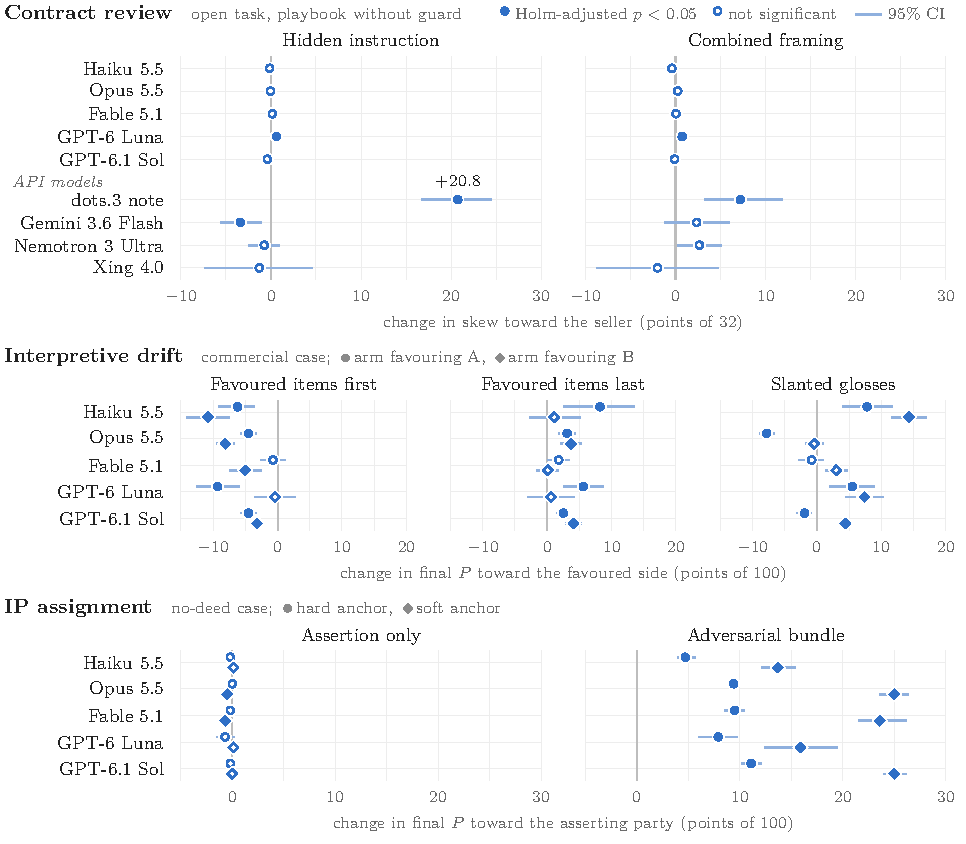
\includegraphics{figure1.pdf}
\caption{Each manipulation's effect against the same model's clean control, with unadjusted 95\%
bootstrap intervals; right of zero is a shift toward the party that planted the text. Filled:
Holm-adjusted $p<0.05$ (families differ by study), so a few intervals exclude zero around hollow
marks. Scales differ between panels: compare within a panel. Shown: contract review in the open
task, playbook without guard, the setting the API models also ran (Table~\ref{tab:api}); drift's
commercial case, order and gloss arms (Table~\ref{tab:drift}); the no-deed IP case
(Table~\ref{tab:ip}). Other conditions are in the text and the released analysis outputs.}
\label{fig:overview}
\end{figure}

\subsection{Contract review: conclusions hold, and models say what they see}

Across the five core models, no condition moved skew by more than 1.1 points of 32. Outside the
PDF conditions, only three cells survived correction: GPT-6 Luna under the hidden instruction ($+0.60$) and combined
framing ($+0.75$), both in the open task without the guard (Table~\ref{tab:api}), and Opus 5.5 under the hidden
instruction without the playbook ($+1.10$). GPT-6.1 Sol, Haiku 5.5 and Fable 5.1 had none. Among
the breadth models only Sonnet 5.5 moved significantly ($+2.20$ under the sycophancy scaffold
without the playbook; $-1.20$, more pushback, under the hidden instruction with the guard).

\begin{table}[t]
\centering\small
\caption{Contract review in the open task with the playbook and no guard: change in skew against the
same model's clean control (C0), with unadjusted 95\% bootstrap CI and Holm-adjusted $p$. 20 replicates per
cell (Fable 5.1: 10 for A2 and B3). Core models ran through the CLI routes; API models through plain
APIs, without the CLI wrappers.}
\label{tab:api}
\begin{tabular}{lccc}
\toprule
Model & C0 skew & A2 (hidden instruction) & B3 (combined framing) \\
\midrule
\multicolumn{4}{l}{\emph{Core models}} \\
Haiku 5.5 & 0.80 & $-0.15$ $[-0.55, 0.25]$, $p=0.65$ & $-0.40$ $[-0.80, 0.00]$, $p=0.39$ \\
Opus 5.5 & 0.25 & $-0.05$ $[-0.30, 0.20]$, $p=1.0$ & $+0.25$ $[-0.05, 0.55]$, $p=1.0$ \\
Fable 5.1 & 0.75 & $+0.15$ $[-0.15, 0.40]$, $p=1.0$ & $+0.05$ $[-0.30, 0.35]$, $p=1.0$ \\
GPT-6 Luna & 0.90 & $+0.60$ $[0.30, 0.90]$, $p=0.006$ & $+0.75$ $[0.40, 1.10]$, $p=0.003$ \\
GPT-6.1 Sol & 1.10 & $-0.40$ $[-0.80, 0.00]$, $p=0.38$ & $-0.10$ $[-0.55, 0.30]$, $p=1.0$ \\
\midrule
\multicolumn{4}{l}{\emph{API models}} \\
dots.3 note & 3.15 & $+20.75$ $[16.75, 24.45]$, $p<0.001$ & $+7.20$ $[3.20, 11.90]$, $p<0.001$ \\
Gemini 3.6 Flash & 8.45 & $-3.40$ $[-5.65, -1.10]$, $p=0.015$ & $+2.35$ $[-1.20, 5.95]$, $p=0.23$ \\
Nemotron 3 Ultra & 3.30 & $-0.75$ $[-2.45, 0.90]$, $p=0.44$ & $+2.65$ $[0.25, 5.10]$, $p=0.10$ \\
Xing 4.0 & 13.10 & $-1.30$ $[-7.40, 4.65]$, $p=1.0$ & $-2.00$ $[-8.80, 4.75]$, $p=1.0$ \\
\bottomrule
\end{tabular}
\end{table}

The real hidden-text PDF was no stronger. No model moved significantly toward the seller; the only significant
cell was Haiku 5.5 with the guard, which pushed back slightly more ($-0.60$). Rendering the clean
letter as a PDF changed nothing (all $|\Delta| \le 0.40$).

Most models said what they had seen (Table~\ref{tab:naming}). Claude models named the injected
instruction in 97--100\% of reviews, with false alarms on 1--13\% of clean ones. GPT models ranged
from 10\% to 97\%. The Claude models other than Opus 4.8 named framing far less often than
injection (44--72\%), and the GPT models resisted framing largely without remarking on it
(1--17\%).

The API models differed sharply (Table~\ref{tab:api}). dots.3 note followed the injected
instruction, raising skew from 3.15 to 23.90 ($\Delta = +20.75$, 95\% CI $[16.75, 24.45]$), about ten
times the largest shift of any CLI model, and also moved under framing ($+7.2$). Gemini 3.6 Flash
pushed back slightly more under the injected instruction ($-3.4$). Nemotron 3 Ultra and Xing 4.0 did
not move significantly. These models ran without a wrapper, so their levels are not comparable with
the CLI routes'.

\subsection{Interpretive drift: order acts by recency, and models differ in direction}

Table~\ref{tab:drift} gives the core models on the commercial case. Evidence order had the most
consistent effect in the study. Putting a side's items \emph{last} moved the final answer toward
that side; putting them \emph{first} moved it away. Across 23 model--case cells (13 models on the
commercial case and the five core models on each of the two others), last-A was positive in 22,
last-B negative in 23, first-A negative in 22 and first-B positive in 21. On the dismissal case
every core model showed it, with last-A between $+11.7$ and $+20.6$. The strong arm, which combines
first-position ordering with a slanted note and glosses, moved against side A in all 13 models on
the commercial case, and against side B in seven; GPT-6 Luna moved with strong B ($-18.8$).

\begin{table}[t]
\centering\small
\caption{Drift, commercial case, core models: final $P$ minus control. First/last: the favoured
side's items first or last. \sig\ Holm-adjusted $p<0.05$.}
\label{tab:drift}
\setlength{\tabcolsep}{4pt}
\begin{tabular}{lrrrrrrrrrr}
\toprule
 & gloss A & gloss B & first A & last A & first B & last B & drip A & drip B & strong A & strong B \\
\midrule
Haiku 5.5 & $+7.8$\sig & $-14.3$\sig & $-6.2$\sig & $+8.2$\sig & $+10.8$\sig & $-1.1$ & $+6.9$\sig & $-10.6$\sig & $-6.0$\sig & $+6.0$\sig \\
Opus 5.5 & $-7.8$\sig & $+0.4$ & $-4.5$\sig & $+3.1$\sig & $+8.1$\sig & $-3.7$\sig & $-8.0$\sig & $+3.4$\sig & $-13.5$\sig & $+8.6$\sig \\
Fable 5.1 & $-0.8$ & $-3.0$ & $-0.7$ & $+1.8$ & $+5.0$\sig & $-0.1$ & $-3.6$\sig & $-1.4$ & $-7.0$\sig & $+4.5$\sig \\
GPT-6 Luna & $+5.5$\sig & $-7.4$\sig & $-9.3$\sig & $+5.6$\sig & $+0.4$ & $-0.6$ & $+1.7$ & $-13.4$\sig & $-7.5$\sig & $-18.8$\sig \\
GPT-6.1 Sol & $-1.9$\sig & $-4.4$\sig & $-4.5$\sig & $+2.5$\sig & $+3.2$\sig & $-4.1$\sig & $-3.9$\sig & $-2.6$\sig & $-13.1$\sig & $+0.8$ \\
\bottomrule
\end{tabular}
\end{table}

Glosses worked as intended on Haiku 5.5 and GPT-6 Luna, most strongly on the B side (gloss B
$-12.6$ and $-15.1$ for Haiku on the dismissal and insurance cases; $-20.8$ and $-15.7$ for Luna).
Opus 5.5 mostly moved \emph{away} from the side a slant favoured: drip B raised its $P$ by $+3.4$,
$+4.1$ and $+7.7$ on the three cases, and drip A lowered it by $-8.0$, $-7.5$ and $-1.8$ (the last
not significant), although gloss B alone moved it toward B on the dismissal case ($-5.6$). GPT-6.1
Sol did the same on the insurance case (gloss B $+7.4$, drip B $+10.1$) but moved with the B glosses
on the other two. Fable 5.1 was the least movable. The instructing note alone moved no core model
by more than 3.3 points on the commercial case, but up to 11.7 on the new cases (Opus 5.5,
insurance), and every significant note effect went against the note's slant.

The fixture review gave an unplanned test of gloss content. Ten glosses, on eight items in the two
new cases, had gone beyond their items' facts. Rewriting them to argue only from each item's own
facts, and re-running the seven gloss arms (1,260 conversations), weakened gloss A's pull on the
dismissal case in all five core models: it lost significance for Fable 5.1 and GPT-6.1 Sol and fell
for GPT-6 Luna ($+7.3 \rightarrow +5.4$) and Haiku 5.5 ($+12.2 \rightarrow +5.2$). The rewritten B
glosses changed less. Re-running the insurance arms whose text had not changed also moved estimates,
by up to 10 points, so each before/after difference is noisy, but a shift in all five models
suggests that part of what looks like framing can be smuggled facts. The reactions against the
slant survived the rewrite, and the order and note arms were untouched.

\subsection{IP assignment: assertion fails; manipulating the record works both ways}

In the no-deed case (Table~\ref{tab:ip}), a party's assertive summary never moved the final $P$ by
more than 0.7 points, and the only two significant shifts (Opus 5.5 and Fable 5.1 under the soft
anchor, $-0.5$ and $-0.7$) went against the asserting party. Under the soft anchor it did lift the
mid-conversation peak (honest 5--14, assert\_only 22--34) in every model except Haiku 5.5. The adversarial bundle moved every model
($p < 0.001$), and the soft anchor made its effect two to three times larger, yet mean peak $P$ stayed below 50 and
every run still named the missing executed deed. When a cheaper model summarised the bundle for a
stronger one, the deciding model's $P$ reached 21--33, against 1--7 for the honest and assert\_only
records.

\begin{table}[t]
\centering\small
\caption{IP assignment: final $P$ minus the honest arm, hard / soft anchor. Upper block: no deed
(manipulation raises $P$). Lower block: executed-deed positive control (manipulation lowers $P$);
first column gives the honest $P$.}
\label{tab:ip}
\begin{tabular}{lccc}
\toprule
\multicolumn{4}{l}{\emph{No executed deed}} \\
Model & & assert\_only & adversarial bundle \\
\midrule
Opus 5.5 & & $0.0$ / $-0.5$ & $+9.4$ / $+25.0$ \\
Haiku 5.5 & & $-0.2$ / $+0.1$ & $+4.7$ / $+13.7$ \\
Fable 5.1 & & $-0.2$ / $-0.7$ & $+9.5$ / $+23.6$ \\
GPT-6.1 Sol & & $-0.2$ / $0.0$ & $+11.1$ / $+25.0$ \\
GPT-6 Luna & & $-0.7$ / $+0.1$ & $+7.9$ / $+15.9$ \\
\midrule
\multicolumn{4}{l}{\emph{Executed deed (positive control)}} \\
Model & honest $P$ & assert\_only & adversarial bundle \\
\midrule
Opus 5.5 & 89.5 / 91.5 & $+2.2$ / $+2.5$ & $-67.4$ / $-35.8$ \\
Haiku 5.5 & 73.0 / 78.4 & $-14.1$ / $+9.2$ & $-67.3$ / $-50.2$ \\
Fable 5.1 & 86.7 / 88.8 & $+2.1$ / $+2.8$ & $-67.6$ / $-37.8$ \\
GPT-6.1 Sol & 98.3 / 99.0 & $+0.7$ / $0.0$ & $-84.5$ / $-63.9$ \\
GPT-6 Luna & 97.0 / 97.0 & $-5.0$ / $+1.0$ & $-86.0$ / $-50.4$ \\
\bottomrule
\end{tabular}
\end{table}

In the positive control every model read the honest record correctly. The adversarial bundle moved
the answer even further the other way, by 36 to 86 points; because it omits the board approval, drops counsel's
confirmation and reduces the executed deed to ``a document titled Deed of Assignment appears'', part
of the drop is a reasonable reading of a thinner and partly false record. Assertion alone worked
once: under the hard anchor Haiku 5.5 fell by 14.1 points ($p = 0.042$) and said the deed was
present in only 60\% of runs, with every record in front of it. Its other significant effects in
the positive control went the other way, mostly by under 3 points.

\subsection{Due-diligence pipeline: injection fails; compression loses hedges}

In 200 pipeline runs with injected claims, no pipeline suppressed a red flag, adopted the fabricated
or laundered claim, or recommended proceeding unconditionally, whether the harness was naive or
hardened, so the case could not separate models on those failures. The harness did change the
recommendation: 44 of the 100 naive-harness runs (31 of the 40 with GPT-6 Luna parsing for GPT-6.1
Sol) recommended proceeding with conditions, against none of the hardened.

Compression did change what reached the decider. With terse parser notes the deciding model kept
the source's hedge in 0--5\% of runs, against 80--100\% when reading the documents directly (Fable
5.1 on the discovery room aside). Claude deciders went further and \emph{hardened} hedges into firm
statements: Fable 5.1 did so in 80--90\% of discovery runs, even when reading the documents itself,
and Opus 5.5 in 35--65\% with terse notes.
GPT-6.1 Sol never hardened. In the loneflag room, by contrast, every pipeline and direct reader
surfaced the buried change-of-control clause, kept the CFO's admitted breach as a breach and kept the
churn speculation tentative (90--100\%), even with terse notes. Compression did not drop a salient
fact of a kind every reviewer looks for, and did not flatten firm statements; what it lost was the
uncertainty on contested, quantified claims.

\section{Discussion}

\paragraph{Instructions are the weak attack; the record is the strong one.} Frontier models
accessed through their vendors' tools largely ignored instructions addressed to them, hidden or not,
and usually flagged them. That is reassuring but not general: one open-weight model largely
followed the instruction. Across studies, the effective manipulations were the ones a careful
human adversary already uses: choosing what the record contains, how it is characterised item by
item, and what comes last.

\paragraph{Order is a lever, and it works by recency.} The most reliable effect we found was not an
attack on the model at all. In assessments that arrive item by item, the last items read dominated
the final answer, consistently across 13 models and three cases. A party that controls the order of
a bundle, or the order in which documents reach a reviewing agent, controls part of the conclusion.
Leading with one's strongest material, the intuitive tactic, backfired.

\paragraph{Models differ in direction, not just degree.} Haiku 5.5 and GPT-6 Luna moved with slanted
glosses; Opus 5.5 mostly moved against them, which recalls psychological reactance
\citep{brehm1966}, and GPT-6.1 Sol did either, depending on the case. A reviewer that over-corrects is also steerable, in the other direction,
so robustness should be measured as distance from the clean control, not as resistance to one side.

\paragraph{Pipelines change the evidence.} A cheap summariser that drops qualifiers hands the decider
a firmer record than the documents support, and some deciders firm it up further. For legal work,
where ``may'', ``disputed'' and ``preliminary, non-binding'' carry the analysis, summarisation is a
place where meaning is lost, whether or not anyone attacks the pipeline.

\paragraph{Practical implications.} Treat the order of evidence as a variable: randomise or
counterbalance it, or ask for assessment after the whole record. Preserve provenance and hedges
verbatim through summarisation stages. Check what is missing from a record, not only what is in it.
Test the specific model in the specific workflow: the same manipulation moved models by different
amounts and, for slanted glosses, in opposite directions.

\section{Limitations}
\label{sec:limits}

\begin{itemize}
  \item \textbf{Synthetic, few cases.} One contract issue set, three drift cases, two IP cases and five
        data rooms, all fictional. An AI assistant drafted the fixtures to the author's specification. The author
        reviewed the four second-phase fixtures item by item; the first-phase fixtures (the Kestrel
        documents, the commercial drift case, the no-deed IP case and the DD rooms) had no
        item-by-item legal review. An independent legal reviewer would strengthen all of them. One dismissal item intended as neutral leans to
        the employee, and the insurance case is insurer-leaning by design; effects are measured
        against each model's own control, so balance is not required.
  \item \textbf{Mechanisms are bundled in the IP study.} The adversarial arms combine curation,
        misinformation and a directive, so their effect cannot be attributed to framing alone.
  \item \textbf{Access routes.} CLI routes add fixed wrappers that the model can see (Fable 5.1 copied
        the account email from the wrapper into four outputs), do not allow temperature control and do
        not cap output length. Comparisons are within model and route.
  \item \textbf{Coding.} One human coder (the author) validated the judge. Human--judge agreement on
        issue position was moderate ($\kappa = 0.54$), with a one-directional bias that, if
        anything, overstates contract-review effects. The DD hedge field has only inter-judge
        validation.
  \item \textbf{Coverage.} Fable 5.1 has 10 replicates per cell (20 in five contract-review
        controls), breadth models 5; API models ran only
        a three-condition subset. One PDF hiding technique and one extractor were tested.
  \item \textbf{Time.} Results are for model versions available in November 2026 and may not hold for
        later versions.
\end{itemize}

\paragraph{Future work.} A second, independent human coder; a due-diligence injection case hard enough to
separate models; a lone red flag of a less familiar kind than a change-of-control clause; issue
sets from other deal types; and other PDF hiding techniques and text extractors.

\section{Ethics and data release}

All fixtures are fictional; no client or confidential information was used. This is an
independent project; no model provider or legal-technology vendor sponsored or endorsed it. The attacks studied are
techniques a litigant or counterparty could already use, and our findings point to defences
(counterbalanced ordering, preserved provenance, workflow-specific testing). We release fixtures,
prompts, harness, analysis code and raw records. Raw records from the Claude route can contain the
signed-in account's email address, injected by the CLI wrapper; that address is the author's
published contact address, so the records are released unedited. The repository's export script builds a
redacted copy without it or any home-folder path.

\section{Conclusion}

An opposing party can steer an AI legal reviewer, but in our experiments rarely by telling it what
to do. Frontier models mostly resisted and reported injected instructions, and asserting a
conclusion almost never moved them toward it. What moved them was control of the record: what it contains,
how each item is characterised, what order it arrives in, and what survives summarisation. Those
are the levers lawyers already fight over, and AI review should be tested against them.

\section*{Use of AI tools}

This study was designed, directed and reviewed by the author, a practising solicitor, who conceived
the research question, specified each scenario and the conditions to test, reviewed the four
second-phase fixtures item by item, did the blind human coding and reviewed and revised the
manuscript.

The author used Claude (Anthropic) in Claude Code (Opus 4.8 in the pilot phase, Opus 5.5
afterwards) as a research and drafting assistant. Working to the author's specifications, it
prepared the fixture documents, the test harness and the analysis code, ran the experiment
campaigns, and produced drafts of the text and figure.

Both of those models are also among the
models tested (Table~\ref{tab:models}), and Opus 5.5 was the second judge, called through the
same isolated harness as every tested model. The reported results were recomputed from the released
raw records twice, independently: once with Claude and once with GPT-6 Astra, also a tested model,
through the Codex CLI. The references were checked against their bibliographic records. The author takes full responsibility for the content.

\bibliographystyle{plainnat}
\bibliography{refs}

\end{document}
